\documentclass[a4paper,11pt]{article}

% --- Encodage et Langue ---
\usepackage[utf8]{inputenc}
\usepackage[T1]{fontenc}
\usepackage[french]{babel}

% --- Mise en page et Typographie ---
\usepackage{geometry}
\geometry{margin=2.5cm, headheight=15pt}
\usepackage{microtype}
\usepackage{lmodern}

% --- Mathématiques ---
\usepackage{amsmath, amssymb}

% --- Images ---
\usepackage{graphicx}
\usepackage{float}

% --- Couleurs et Boîtes ---
\usepackage{xcolor}
\definecolor{primary}{RGB}{0, 85, 150}      % Bleu technique
\definecolor{secondary}{RGB}{240, 248, 255} % Bleu très clair pour les fonds
\definecolor{solcolor}{RGB}{245, 250, 245}  % Vert très clair pour les solutions
\definecolor{solframe}{RGB}{60, 120, 60}    % Vert foncé pour les bordures de solution
\definecolor{vhdlkeyword}{RGB}{0, 0, 180}   % Bleu pour mots-clés VHDL
\definecolor{vhdlcomment}{RGB}{0, 128, 0}   % Vert pour commentaires
\definecolor{vhdlstring}{RGB}{163, 21, 21}  % Rouge pour chaînes

\usepackage{tcolorbox}
\tcbuselibrary{skins}
\usepackage{caption} % Pour \captionof à l'intérieur des boîtes

% --- Tableaux professionnels ---
\usepackage{booktabs}
\usepackage{array}

% --- Affichage de code VHDL ---
\usepackage{listings}
\lstdefinestyle{vhdlstyle}{
    language=VHDL,
    basicstyle=\small\ttfamily,
    keywordstyle=\color{vhdlkeyword}\bfseries,
    commentstyle=\color{vhdlcomment}\itshape,
    stringstyle=\color{vhdlstring},
    numbers=left,
    numberstyle=\tiny\color{gray},
    numbersep=8pt,
    frame=single,
    framerule=0.5pt,
    rulecolor=\color{gray!50},
    backgroundcolor=\color{gray!5},
    breaklines=true,
    columns=fullflexible,
    showstringspaces=false,
    tabsize=4,
    inputencoding=utf8,
    morekeywords={entity,is,port,in,out,architecture,of,begin,end,signal,process,variable,constant,type,component,if,then,else,elsif,case,when,for,loop,while,generate,map,and,or,not,xor,nand,nor,xnor,library,use,all,std_logic,std_logic_vector,std_ulogic,std_ulogic_vector,integer,boolean,bit,bit_vector,real,time,character,severity_level,file_open,file_close,read,write,wait,assert,report,null,transport,inertial,after,rising_edge,falling_edge,to,downto,others,range,reverse_range,attributes,function,procedure,return,exit,next,record,units,array,unsigned,signed,ieee,numeric_std}
}
\lstset{style=vhdlstyle}

% --- Titres ---
\usepackage{titlesec}
\titleformat{\section}
  {\color{primary}\Large\bfseries}
  {\thesection}{1em}{}[\titlerule]
\titleformat{\subsection}
  {\color{primary}\large\bfseries}
  {\thesubsection}{1em}{}

% --- Gestion des solutions (Mettre \solutionsfalse pour cacher les solutions) ---
\newif\ifsolutions
\solutionstrue % <--- Changez en \solutionsfalse pour la version étudiant

\newtcolorbox{notebox}{
  colback=secondary,
  colframe=primary,
  fonttitle=\bfseries,
  title=Notes et Conseils,
  arc=4pt,
  boxrule=0.8pt
}

\newtcolorbox{questionbox}{
  colback=secondary,
  colframe=primary,
  fonttitle=\bfseries,
  title=Questions,
  arc=4pt,
  boxrule=0.8pt
}

\newtcolorbox{solbox}{
  colback=solcolor,
  colframe=solframe,
  fonttitle=\bfseries,
  title=Solution,
  arc=4pt,
  boxrule=0.8pt
}

% --- Titre du document ---
\title{\textcolor{primary}{\Huge\bfseries TD VHDL 2/3 -- Électronique Numérique}\\[0.5em] \Large Circuits séquentiels et Automates}
\author{}
\date{}

\begin{document}

\maketitle
\vspace{-2em}

\begin{notebox}
\textbf{Remarque :} Ce TD constitue la suite de l'introduction à la description matérielle en VHDL. Il aborde les circuits séquentiels (compteurs) et la description d'automates aux niveaux logique et RTL. Il est conseillé de tester les codes sur un simulateur (GHDL) pour valider vos acquis.
\end{notebox}

\vspace{1em}

\section{Descriptions de chemin de données séquentiel}

\begin{questionbox}
\begin{enumerate}
    \item Coder en VHDL au moins deux architectures numériques qui réalisent un compteur, qui compte de 0 à 255, en respectant l'entité donnée ci-dessous. On note que les opérandes sont codés en \textbf{unsigned(7 downto 0)} (octets non-signés). On prendra soin de \underline{dessiner} le circuit \underline{avant} de coder l'architecture.
    \item Tester le circuit à l'aide du testbench fourni.
\end{enumerate}
\end{questionbox}

\ifsolutions
\begin{solbox}
On présente 2 architectures, {\it in fine} identiques, mais codées différemment. L'architecture 2 semble plus naturelle ; l'architecture 1 sépare explicitement partie combinatoire et partie séquentielle.

\vspace{0.5em}
\centering
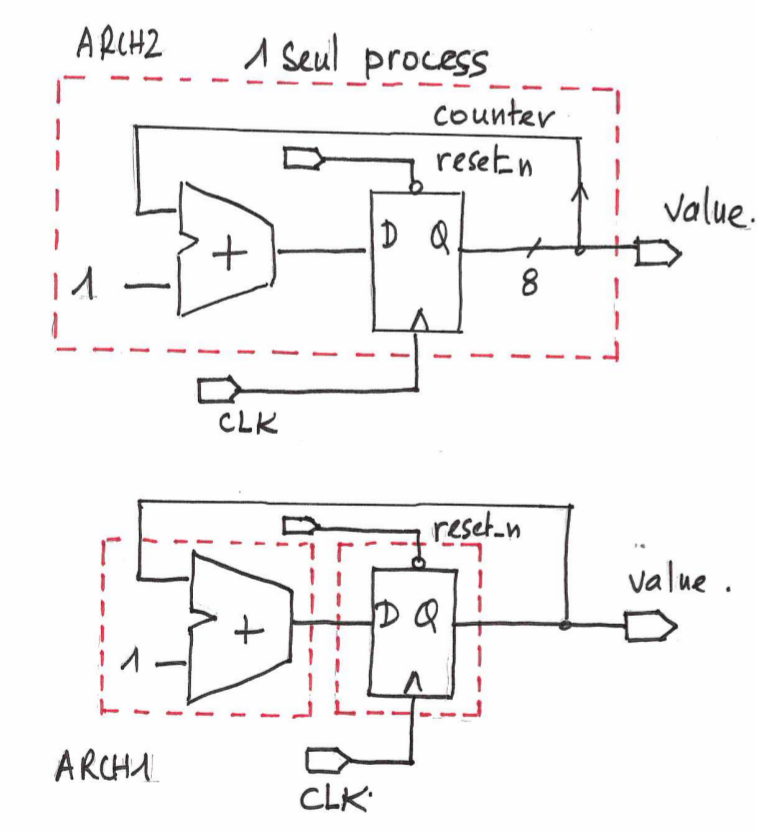
\includegraphics[width=6cm]{./compteur.png}
\captionof{figure}{Architecture du compteur, deux organisations de code possibles : soit 1 seul processus, soit 2 processus (1 processus + 1 assignation concurrente)}
\label{compteur}

\vspace{1em}
\lstinputlisting[language=VHDL]{./code/compteur.vhd}
\end{solbox}
\fi

\section{Descriptions d'automates au niveau logique}

Soit un automate bien connu des informaticiens parisiens, sur la figure \ref{iloveparis}.

\begin{figure}[H]
\centering
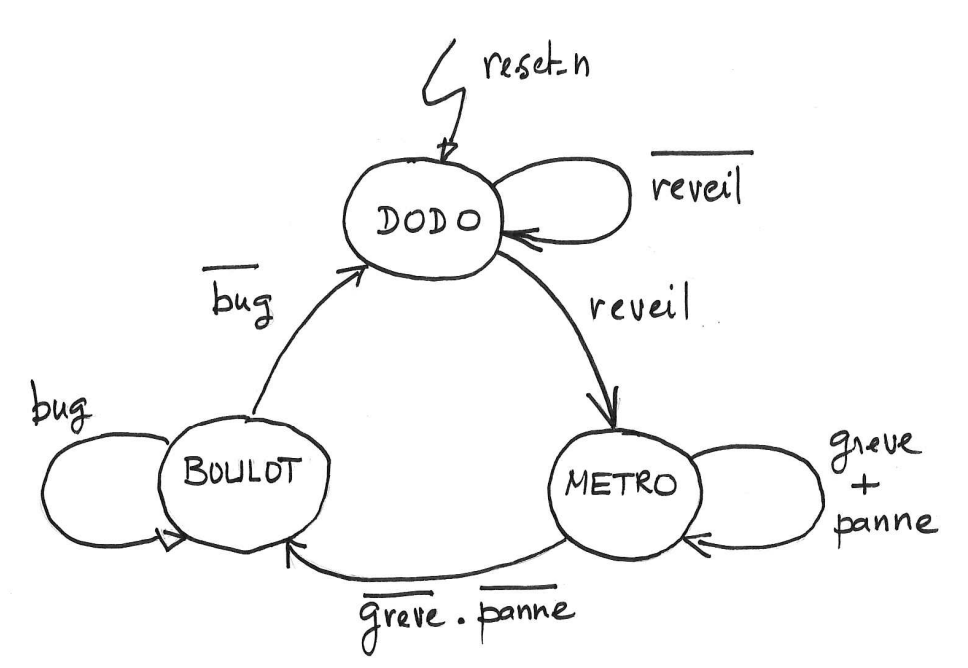
\includegraphics[width=8cm]{./iloveparis.png}
\caption{Diagramme états-transitions de l'automate "I love Paris"}
\label{iloveparis}
\end{figure}

\begin{questionbox}
\begin{enumerate}
    \item Vérifier que, dans le cas d'un encodage one-hot, les équations d'état suivant sont bien données par :
    $$
    \left\{
    \begin{array}{rl}
    D_0 &= Q_0.\overline{reveil}+Q_2.\overline{bug} \\
    D_1 &= Q_0.reveil+Q_1.(greve+panne)\\
    D_2 &= Q_1.\overline{greve}.\overline{panne}+Q_2.bug\\
    \end{array}
    \right.
    $$
    \item Coder l'automate "I\_love\_Paris" en VHDL, au niveau logique, en prenant soin de bien coder les bascules D à l'aide de processus. Respectez l'entité fournie ici. On utilisera une assignation conditionnelle (when) pour coder le signal de sortie "up\_and\_running".

    \lstinputlisting[language=VHDL]{./code/i_love_paris_entity.vhd}

    \item Utilisez le testbench donné sous Moodle pour tester votre automate. Observez le résultat.
\end{enumerate}
\end{questionbox}

\ifsolutions
\begin{solbox}
\lstinputlisting[language=VHDL]{./code/i_love_paris_logic.vhd}
\end{solbox}
\fi

\section{Descriptions d'automates au niveau RTL}

Ce niveau d'abstraction RTL est le plus couramment utilisé, car il permet de s'affranchir des détails des équations logiques, et décrire des automates (et {\it micro-architectures}) de manière plus naturelle.

Le niveau RTL repose sur la notion d'{\it inférence matérielle} : l'Électronicien doit connaître certains {\it motifs de conception}\footnote{"Design patterns", en anglais.}, afin de permettre à l'outil de synthèse d'établir automatiquement les équations logiques sous-jacentes.

Le cas des automates d'états finis est instructif en ce sens. Voici un exemple de codage VHDL, qui décrit un automate, sans expliciter les équations logiques sous-jacentes, ni l'encodage des états. Pour information, le synthétiseur peut choisir de lui-même un encodage qui maximise la fréquence de fonctionnement du circuit (encodage one-hot généralement), ou tout autre type de contraintes imposées par le concepteur.

\subsection*{Exemple d'automate de niveau RTL}

Nous donnons ici à titre d'exemple un diagramme états-transitions, ainsi que son code VHDL de niveau RTL. Notez que nous avons séparé le processus ici appelé "next\_state\_p", qui code la fonction de transition (calcul de l'état suivant), et la sortie de l'automate.

\begin{center}
\begin{minipage}[t]{8cm}
\vspace{0pt}
\lstinputlisting[language=VHDL]{./code/automate.vhd}
\end{minipage}%
\begin{minipage}[t]{7cm}
\vspace{40pt}
\centering
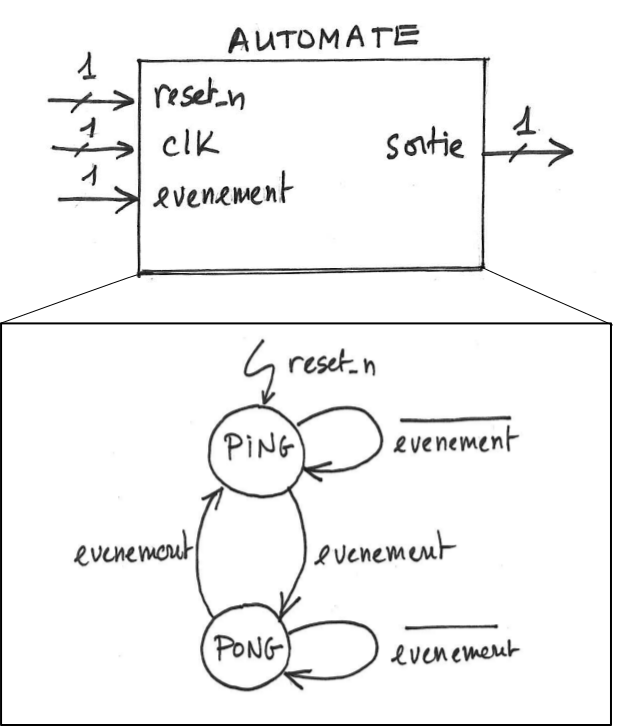
\includegraphics[width=6cm]{./ent_arch_ping_pong.png}
\end{minipage}
\end{center}

\begin{questionbox}
\begin{enumerate}
    \item Prenez le temps de comprendre le codage utilisé ici.
    \item Coder l'automate "I\_love\_Paris" en VHDL, au niveau RTL, en vous inspirant de l'exemple donné.
    \item Utilisez le même testbench que précédemment pour tester votre automate. Modifier uniquement le nom de l'architecture associée à l'entité instanciée.
\end{enumerate}
\end{questionbox}

\ifsolutions
\begin{solbox}
\lstinputlisting[language=VHDL]{./code/i_love_paris.vhd}

\vspace{1em}
\centering
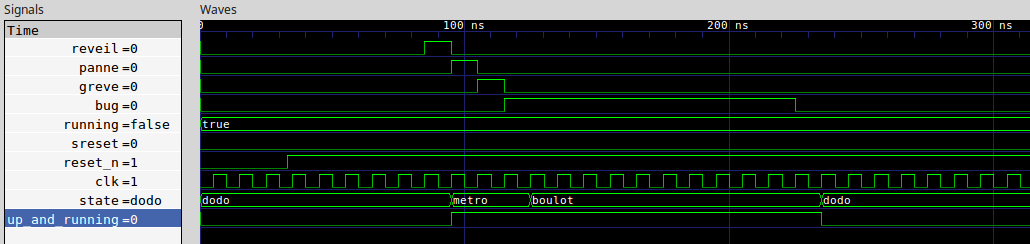
\includegraphics[width=16cm]{./metro_boulot_dodo_chrono.png}
\captionof{figure}{Chronogramme de simulation de l'automate "I love Paris"}
\end{solbox}
\fi

\end{document}
